\documentclass[17pt, a4paper]{extreport}
\usepackage{graphicx}

\begin{document}
\chapter[Introduction]{Introduction}
\section[Voltage sag]{Voltage sag}
\paragraph{}
Voltage sag is one of the most significant power quality sues that can affect the majority of sensitive equipments like personal computers (PC), adjustable speed drives (ASD), programmable logic controllers (PLC). Voltage sag is defined as a decrease in rms voltage or current at the power frequency for durations of 0.5 cycle to 1 min. Typical values are from 0.1 to 0.9 pu.[IEEE Recommended Practice for Evaluating Electric Power System Compatibility With Electronic Process Equipment]. Voltage sags are present in power systems, but only during the past decades customers are becoming more sensitive to the inconvenience caused [Pirjo Heine and Matti Lehtonen, “Voltage sag distributions caused by power systems faults,” IEEE Transactions on Power Systems, vol.18, No.4, pp.1367-1373, November 2003]. Voltage sag can cause serious problems to sensitive loads, because these loads often drop off-line due to voltage sag. Out of the various disturbances that effect the power quality, voltage sag happens to be the most frequent disturbance. If a voltage sag occurs for a longer duration it is called an undervoltage. 
\paragraph{}
\textbf{Characteristics of Voltage sags:}
\begin{enumerate}
    \item 	\textbf{Magnitude}:- The minimum value of Vrms(1/2) recorded during a voltage sag. The magnitude is expressed as a value in volts or as a percentage or per-unit value of the declared voltage or sliding-reference voltage.[ IEEE Guide for Voltage Sag Indices]
    
    \item 	\textbf{Duration}:- The voltage sag duration is nothing but the period of time in which the voltage is lower than the stated limit; normally sag duration is less than 1 second [IEEE Std. 493, 1997]. The voltage sag starts when at least one of the rms voltages drops below the sag-starting threshold. The sag ends when all three voltages have recovered above the sag-ending threshold.
    
    \item \textbf{Unbalance of sag}:- In the power system the faults are classified as symmetrical (balanced) and unsymmetrical (unbalanced) depending on the type of fault. If three phase fault occurs, the sag will be symmetrical but if the fault is single phase, double phase or double phase to ground faults the sag in three phases will not be symmetrical.
    
    \item 	Point on wave of sag initiation.
    
\end{enumerate}

\textbf{Types of Voltage Sag:}
\begin{enumerate}
    \item \textbf{Single phase sags}:- These are frequently occurring voltage sags and are basically due to the phase to ground faults.
    
    \item \textbf{Phase to phase sags:} The two phase or phase to phase sags are caused by tree branches, adverse weather, animals or vehicle collision with utility poles.
    \item \textbf{Three phase sags:} - These sags are caused by switching or tripping of a 3 phase circuit breaker.These sags are caused by switching or tripping of a 3 phase circuit breaker, switch or recloser which will create three phase voltage sag on other lines fed from the same substation.
    
    
\end{enumerate}

\textbf{Following are some of the causes for the occurrence of voltage sag:-}\begin{enumerate}
    \item Starting of motors can cause a voltage sag as a large amount of current will be drawn during starting when compared to current drawn while running at rated speed.
    
    \item Excessive or sudden load changes can cause a voltage sag.
    
    \item 	When a fault occurs there will be voltage sag until the protective switch gear operates.
\end{enumerate}

\section[Voltage Tolerance Curves]{Voltage Tolerance Curves}
\subsection{Automatic Speed Drives:} An ac ASD controls the speed of an induction or synchronous motor by converting fixed frequency/fixed magnitude ac mains supply voltage to a variable frequency/variable magnitude voltage at the motor terminals.  The ASDs are three-phase equipment and d ifferent combinations of three phase voltages during the sags have different effects on their operation. Testing of ASDs was conducted with the following three types of voltage sags:

\begin{enumerate}
    \item Three-phase balanced voltage sags.
    \item Generalized two phase voltage sag.
    \item Generalized single phase voltage sag.
\end{enumerate}

 To illustrate this, the test procedure used with rectangular voltage sags is described: 
 
 \begin{enumerate}
     \item The drive was first connected to the voltage sag generator (VSG) which supplies the drive with rated input characteristics. Controlled motor was started unloaded.
     
     \item The motor was loaded with one of three load types and the selected torque. The speed of the motor was adjusted to one of the pre-selected values. One of three voltage sag types was selected for testing. The point on wave of the sag initiation and phase shift during the sag were set.
     
     \item Voltage sags were applied in steps of 1\% of rated value, starting from 0 V. For each sag magnitude, the duration of
the sag was prolonged until some of drive protection systems activate the disconnection of the drive, or, if there is no disconnection, up to a few seconds. The critical sag duration was ascertained by up to 10 repeated measurements. A 5–10 s recovery time was allocated between the consecutive voltage sags.

\item In testing with sags for which voltage in the unsagged phase(s) was used as a parameter, this value was changed in 10\% steps from 0–100\% of the rated value, and measurements described in step 3 were repeated.

\item The point onwave of voltage sag initiation was adjusted in steps of $15^{o}$ (from 0 to $360^{o}$) and measurements described in step 3 were repeated.

\item The phase shift during the sag was changed in steps of 15 (from 0 to ±$90^{o}$) and measurements described in step 3 were repeated. 

\item The speed of the motor was changed to the next value and measurements described in step 3 were repeated (motor speeds selected for testing were: 100, 75, 50, and 25\% of rated motor speed).

\item Loading torque was changed to the next value, and measurements described in step 3 were repeated. Torque values selected for testing were: 100, 75, 50, 25, and 0\% of rated motor torque.

\item The load typewas changed to next of three types (i.e., constant torque load, load with linear relationship between the speed and torque, and load with quadratic relationship between the speed and torque) and measurements described in step 3 were repeated.

\item The voltage sag type was changed to the next of the three types and measurements described in step 3 were repeated.


 \end{enumerate}
 
 \begin{figure}
     \centering
     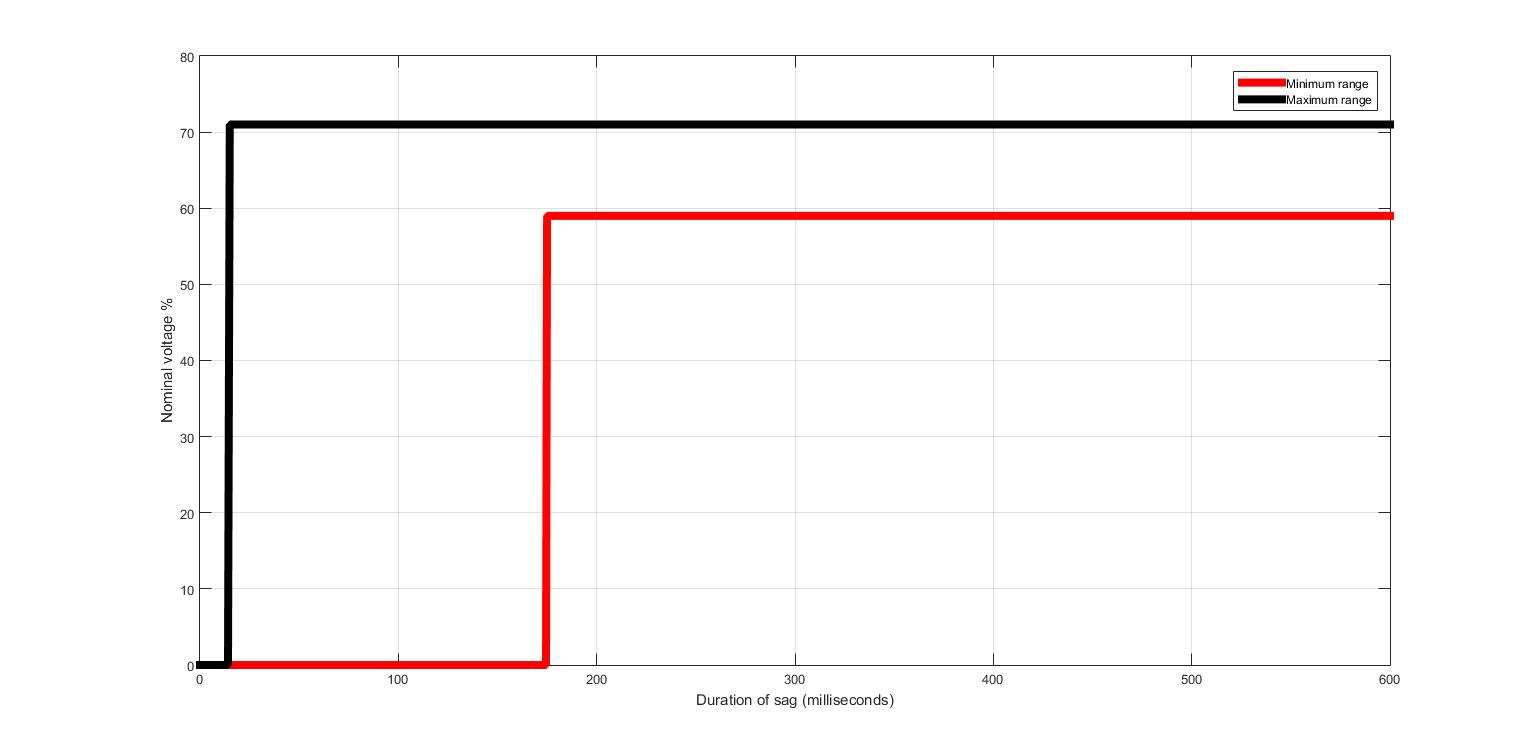
\includegraphics[width = \textwidth]{asd2.jpg}
     \caption{Single graph representation of drive sensitivity to various types of voltage sags}
     \label{fig:asd_characteristics}
 \end{figure}

\subsection{Personal computers (PCs)} Personal computer (PC) is a a general-purpose, rather complex electronic computing device designed to be operated by one person at a time. PCs can be implemented as “real-time” systems (i.e., for real-time control of various external devices), for online control of communication between two or more locations, or as a part of continuous process-control applications. Two software malfunction criteria that may result in different voltage-tolerance curves for PCs were considered in the tests: a) lockup of a read/write operation, and b) blockage of the operating system (OS). Tests were performed with rectangular voltage sags and an ideal voltage supply, as well as with nonrectangular sags occurring during the start of the large motors. The following procedure was used in tests with rectangular voltage sags.

\begin{enumerate}
    \item The computer (with all input/output (I/O) and pointing devices connected) was switched on and allowed to boot and load the operating system.
    
    \item Read/write operation (copying of different files from CD-ROM to the computer’s hard drive) was initiated.
    
    \item Voltage sags were applied in steps of 1\% of rated voltage, starting from 0 V. The point on wave of the sag initiation and the phase shift during the sag were both kept constant. For each voltage sag magnitude, the duration of the sag was progressively increased until lockup of copying operation was obtained, or the operating system was blocked, or the computer was forced to restart, or if none of the former happened up to a few seconds. The critical sag duration for each of these hardware/software criteria was ascertained by up to ten repeated measurements for each value of the sag magnitude. In cases when the tested computer had different sensitivities to voltage sags with respect to different software/hardware criteria, it would first lock up the read/write operation, then it would block the OS, and, finally, it would restart. A recovery time of 5-10 s was allocated between the consecutive voltage sags.
    
    \item The point on wave of voltage sag initiation was adjusted in steps of $15^{o}$ (from 0 to $360^{o}$) and the  measurements described in Step 2 were repeated.
 \item  The phase shift during the sag was changed in steps of 15 (from 0 to $90^{o}$ ) and the measurements described in Step 3 were repeated.
 
 \begin{figure}
     \centering
     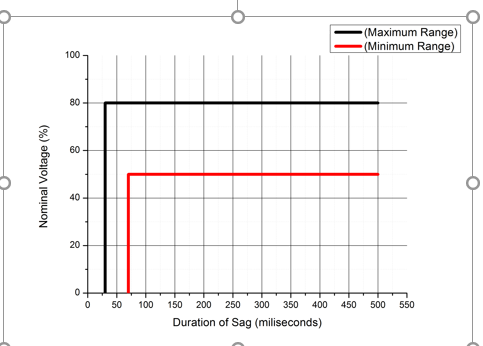
\includegraphics[width=\textwidth]{pc.PNG}
     \caption{ Voltage tolerance curve for Personal Computer}
     \label{fig:PC_characteristics}
 \end{figure}
 
 \subsection{AC Coil Contactors:} Switching elements are necessary for efficient control, isolation, protection, and signaling in all electrical systems. Out of all the other switching elements contactors make possible the centralized or remote control of motors and other industrial machinery. They can be integrated easily with other important circuits to perform more complex functions such as coordinated protection, time-dependent operation, or factory automation. Contactors are designed to disconnect the load or circuit they control when the main power supply (control voltage) is interrupted. While testing AC Coil Contactors. Tests were performed with rectangular voltage, an ideal voltage supply, and also with two-stage sags and with sags due to the starting of large motor. The testing of the contactors was always conducted according to a well-defined procedure. For example, the procedure for testing with rectangular voltage sags proceeds as follows.
 \begin{enumerate}
     \item The contactor’s main electrical contacts are engaged by applying nominal voltage to the ac coil terminals (by pressing
the “ON” button).
\item Keeping constant the values of the point on wave of sag initiation and phase shift during the sag, voltage sags are applied in steps of 1\% of nominal voltage, starting from 0 V. For each voltage sag magnitude, the duration of the sag is progressively increased until contactor disengages, or up to a few seconds. The sag duration required for disengagement is ascertained by ten repeated measurements for each sag magnitude, point on wave of initiation and phase shift. After each disengagement, a minimum of 5-s recovery time is allocated before the next voltage sag is applied. 
\item The point on wave of voltage sag initiation is adjusted in steps of $15^{o}$ (from 0 to $360^{o}$) and the measurements described
in step 2 are repeated.
\item The phase shift during the sag is changed in steps of $15^{o}$ (from 0 to $90^{o}$) and the measurements described in step 2 are
repeated. 
\end{enumerate}
 \begin{figure}
     \centering
     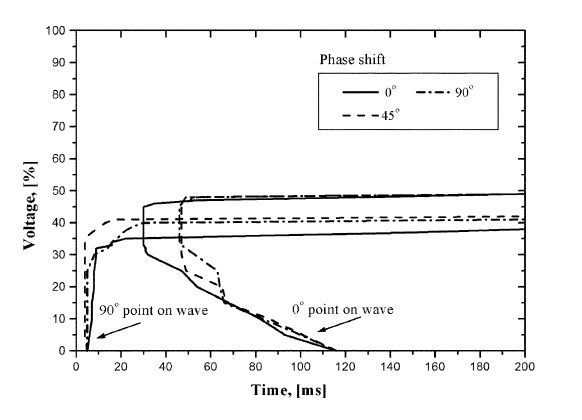
\includegraphics[width=\textwidth]{contactor.png}
     \caption{Contactor Characteristics}
     \label{fig:contactor_characteristics}
 \end{figure}
 \subsection{Programmable Logic Controller (PLCs) } PLCs (Programmable Controllers) have been utilized widely as the automation backbone of industrial process sectors such as mechanical manufacturing, coal mine, chemical industry, power engineering and so on[ Chen Zhuo “Exploring the Application of Programmable Logic Controller (PLC) [J]” Electronics Word, no. 23, pp. 174-177, Dec., 2015]. This is an important category of equipment for industrial processes because the entire process is often under the control of these devices. The sensitivity to voltage sags varies greatly but portions of an overall PLC system have been found to be very sensitive. 
 
 \begin{figure}
     \centering
     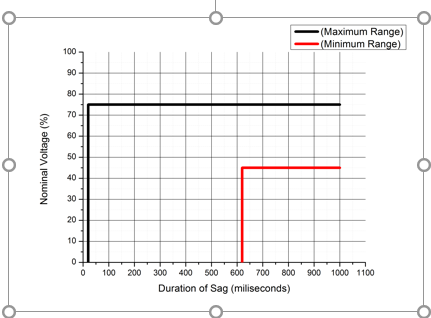
\includegraphics[width=\textwidth]{plc.PNG}
     \caption{Voltage tolerance curve for PLC}
     \label{fig:my_label}
 \end{figure}
 
 \subsection{5 HP AC Drive} This AC drive controls the speed of an induction or synchronous motor by converting fixed frequency/fixed magnitude ac mains supply voltage to a variable frequency/variable magnitude voltage at the motor terminals. Testing of 5 HP AC Drive is similar to the testing of ASD. After performing the tests we get the voltage tolerance curve of the 5 HP AC Drive
 \begin{figure}
     \centering
     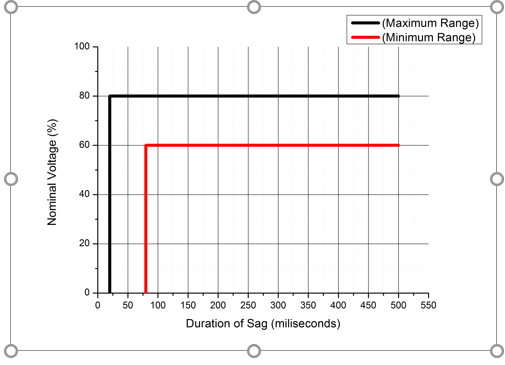
\includegraphics[width=\textwidth]{5hpacdrive.PNG}
     \caption{Voltage tolerance curve for 5 HP Ac Drive}
     \label{fig:5hp_ac_drive}
 \end{figure}
 \subsection{Motor Starter}The voltage tolerance curves for the motor starter after performing the tests is attached \ref{fig:motor_starter}.
 \begin{figure}
     \centering
     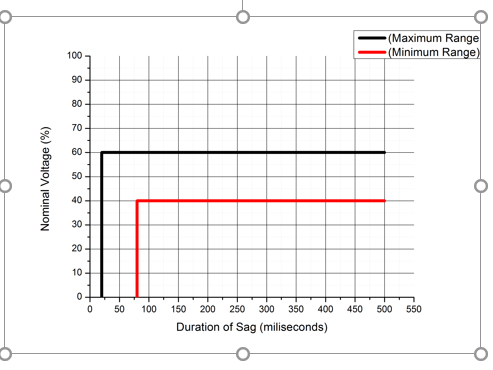
\includegraphics[width=\textwidth]{motorstarter.PNG}
     \caption{Motor Starter}
     \label{fig:motor_starter}
 \end{figure}

\end{enumerate}
\end{document}
